\section{Integration Tools}
\label{sec:integration}
\subsection{Darshan}
Darshan is divided into two main parts: 1) \emph{darshan-runtime} which contains the instrumentation of the characterization tool and produces a single log file a the end of each execution summarizing the I/O access patterns used by the application~\cite{darshan-doc}. 2) \emph{darshan-util} which is intended for analyzing log files produced by darshan-runtime~\cite{darshan-doc}. The \Darshan focuses on the \emph{darshan-runtime}~\cite{darshan-runtime} as this is where the source code of I/O event data is recorded by Darshan.

Darshan tracks the start, duration and end time of an application run via the C function \emph{clock\_gettime()} and converts the result into seconds and passes the result to a struct that is then used to report the summary log files~\cite{darshangithub}. Therefore, in order to retrieve the \emph{absolute timestamp} and include it into the I/O event data during run time, a time struct pointer was added to the function call that used \emph{clock\_gettime()} in \emph{darshan-runtime}. This pointer was passed through all of Darshan's modules and the \emph{absolute timestamp} was collected. This was the preferred method as it required minimal changes to Darshan's source code and no additional overhead and latency between the function call and recording of the \emph{absolute timestamp}. 

\begin{figure}
	\centering
	%\includegraphics[trim=0.2cm 8.5cm 12cm 0cm ,clip,width=0.9\linewidth]{figs/fig_kokkos_ldms.pdf}
	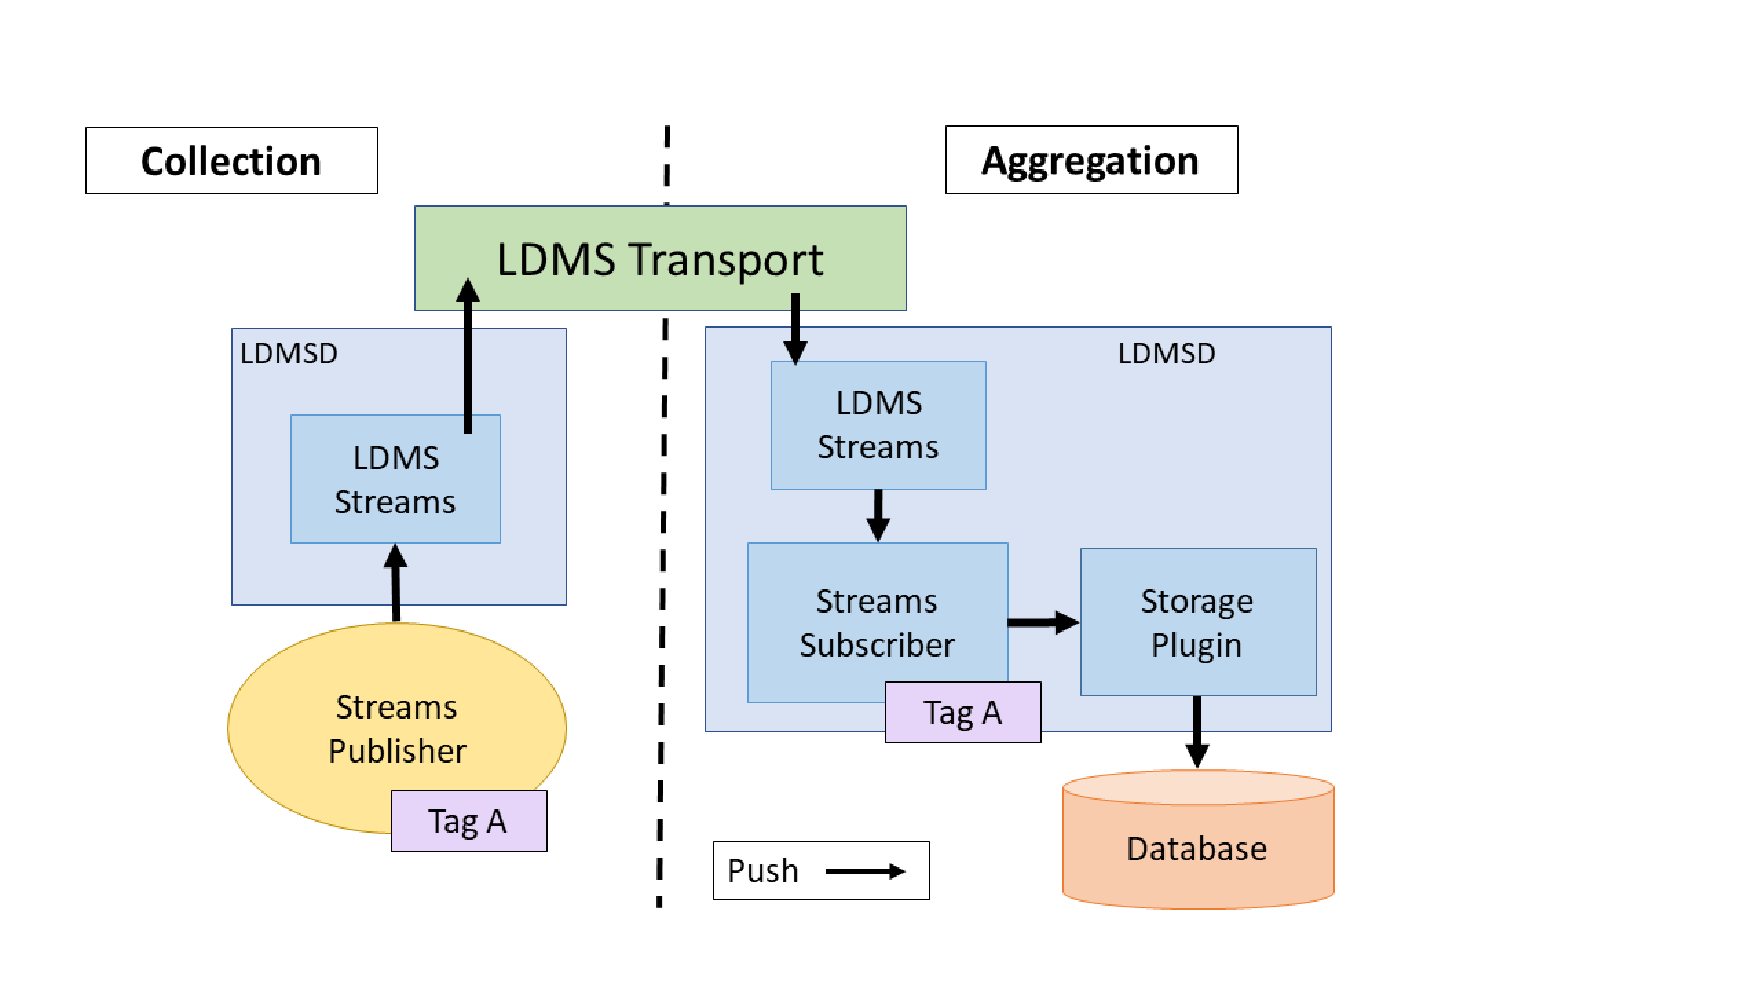
\includegraphics[trim=0 1cm 1 1.5cm ,clip,width=1.2\linewidth]{figs/ldms-overview.pdf}
	\caption{Overview of the LDMS event data collection. Application data is \emph{pushed} by publishing data to the \emph{LDMS Streams} which is then \emph{pushed} through the LDMS transport to the \emph{LDMS Streams} LDMS aggregator (right) where the data is \emph{pushed} to the streams subscriber (Tag A) and stored to a database.}
	\label{f:LDMS Overview}
\end{figure}

\subsection{LDMS Streams}
The word, \emph{LDMSD}, refers to an LDMS daemon that provides the capability of data collection, transport and storage and their \emph{plugins} determine the functionality of these capabilities~\cite{ldmsgithubwiki}. Daemons on the compute nodes run sampler plugins and transport is achieved through multi-hop \emph{aggregation}. LDMS had two levels of aggregator daemons~\cite{ldmsgithubwiki}which can utilize storage plugins to store any sets of data into various formats so long as it's specified beforehand.

\begin{figure}
	\centering
	%\includegraphics[trim=0.2cm 8.5cm 12cm 0cm ,clip,width=0.9\linewidth]{figs/fig_kokkos_ldms.pdf}
	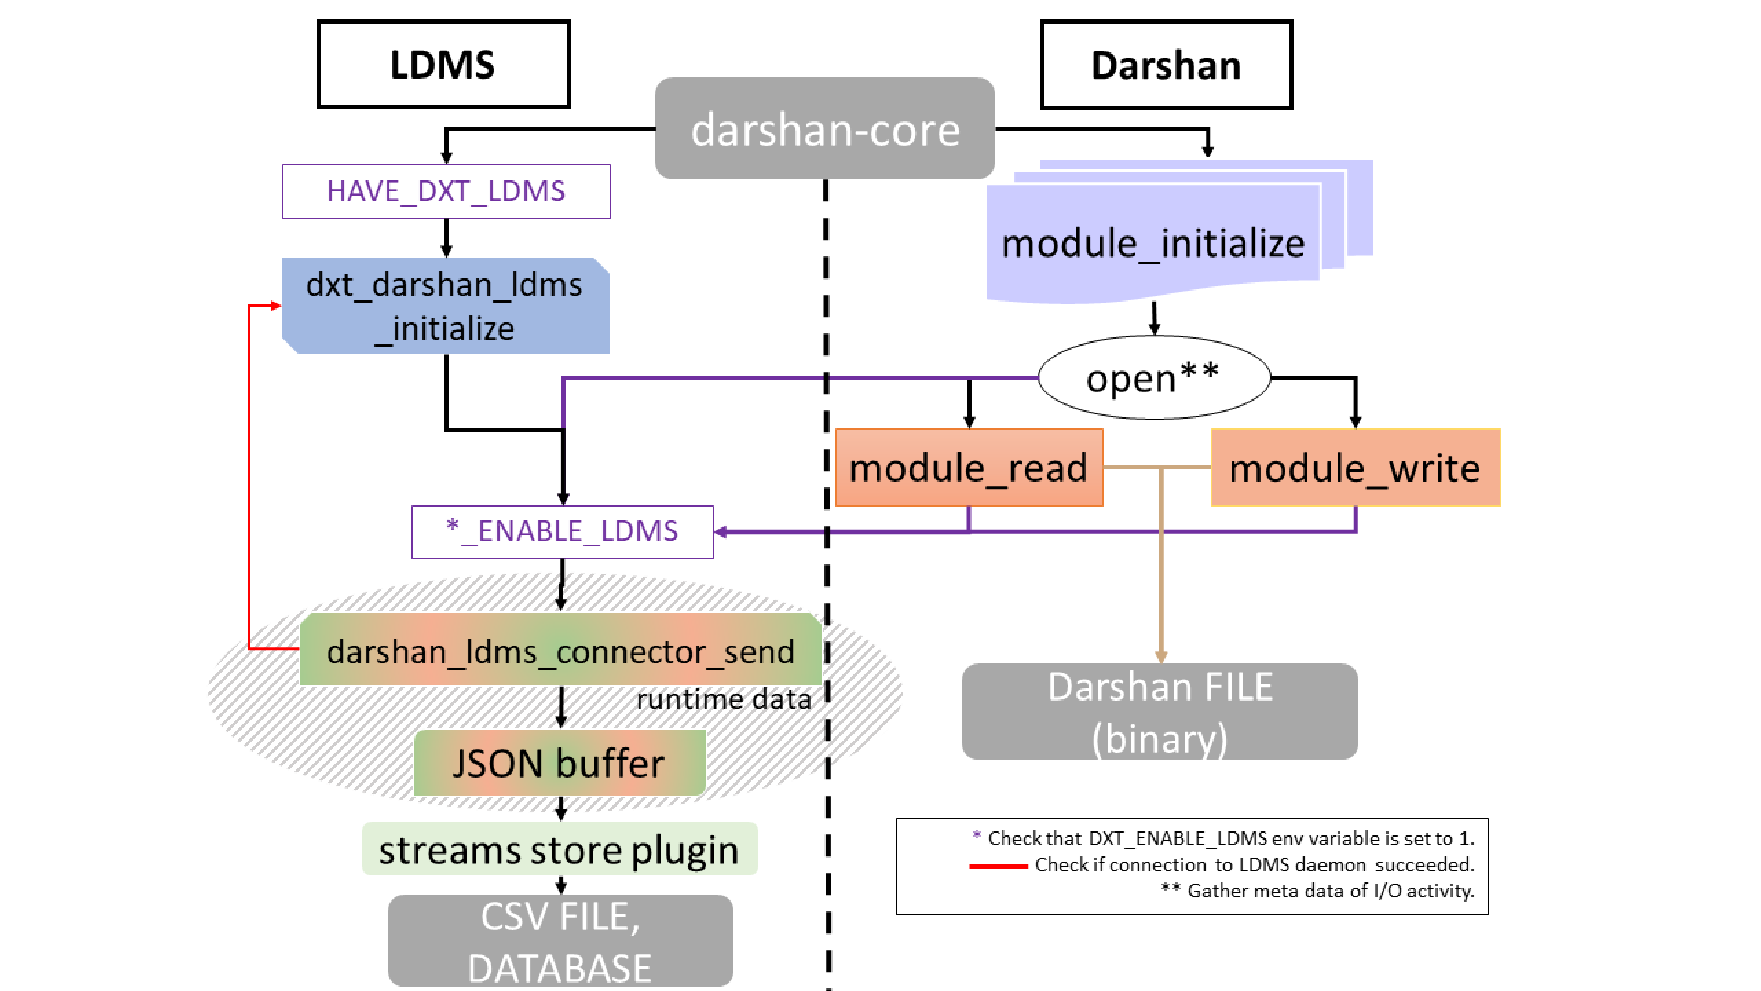
\includegraphics[trim={3.5cm 0 0 0},clip,
	width=1.15\linewidth]{figs/darshan-connector.pdf}
	\caption{Overview of the \connector design and how it collects I/O data for each read, write, open and close events per rank from Darshan. The LDMS library must be linked against the Darshan build in order to utilize the \emph{LDMS Streams} functionality and store plugins.}
	\label{f:Darshan Connector}
\end{figure}

The \Darshan leverages the LDMS transport to support the injection and transport of application I/O data which requires a \emph{push-based} method to reduce the amount of memory consumed and data loss on the node as well as reduce the latency between the time in which the event occurs and when it is recorded. A \emph{pull-based} method would require a buffering to hold an unknown number of events between pulls. Also, the transported data format needs to support  \emph{variable-length} events because the I/O data may will most likely vary in size. 

This leads to the LDMS \emph{publish-subscribe bus} capability , \emph{LDMS Streams}, which has been enhanced to support I/O event data. This capability is intended for publishing and subscribing to an \emph{LDMS streams tag}. The tag needs to be specified in LDMS daemons and \emph{plugins} in order to publish event data to \emph{LDMS Streams} and receive this published \emph{LDMS Streams} data that match the tag.This process and the \emph{push-based} method can be seen in Figure~\ref{f:LDMS Overview}. Event data can be specified as either \texttt{string} or \texttt{JSON} format. The \emph{LDMS Streams} API was modified to support long application connections and message injections. \emph{LDMS Streams} uses best effort without a reconnect or resend for delivery and does not cache it's data so the published data can only be received after subscription. The \emph{LDMS Streams} allows the ability for any data source to be injected into the LDMS transport.

\subsection{Darshan Connector}

The most recent version of Darshan allows for full tracing of application I/O workloads using their DXT instrumentation module which can be enabled and disabled as desired at runtime. DXT provides high-fidelity traces for an application's I/O workload vs Darshan's traditional I/O summary data and currently traces POSIX and MPI-IO layers~\cite{darshan-runtime}. This design leverages the additional I/O tracing Darshan's DXT provides through the new \connector capability.


The \connector functionality collects both DXT data and Darshan's original I/O data and optionally publishes a message in JSON format to the \emph{LDMS Streams} interface as seen in Figure 3. The \emph{absolute timestamp} is also included in this message with the given name "timestamp". The LDMS transport then transports the I/O event data to a \emph{DSOS} database where Grafana can access and query this data. the \connector currently uses a single unique \emph{LDMS Stream tag} for this data source. For the file level accesses that DXT does not trace or for file level access type that have different name-value pairs, a value of "N/A" or "-1" is given in the JSON message. 

Darshan has a large number of metrics it uses for I/O tracing and
post-processing calculations. The current stages of this framework
collects a subset of these metrics to publish to \emph{LDMS Streams},
as presented in Figure \ref{f:CSV Header and Output}. These metrics
provide the most value to the user as they will provide the ability to
create new I/O behavior analyses and visualizations to get further
insights of the application I/O behavior, and reveal correlations
between I/O performance variability and system behavior.
\begin{figure}
	\centering
	%\includegraphics[trim=0.2cm 8.5cm 12cm 0cm ,clip,width=0.9\linewidth]{figs/fig_kokkos_ldms.pdf}
	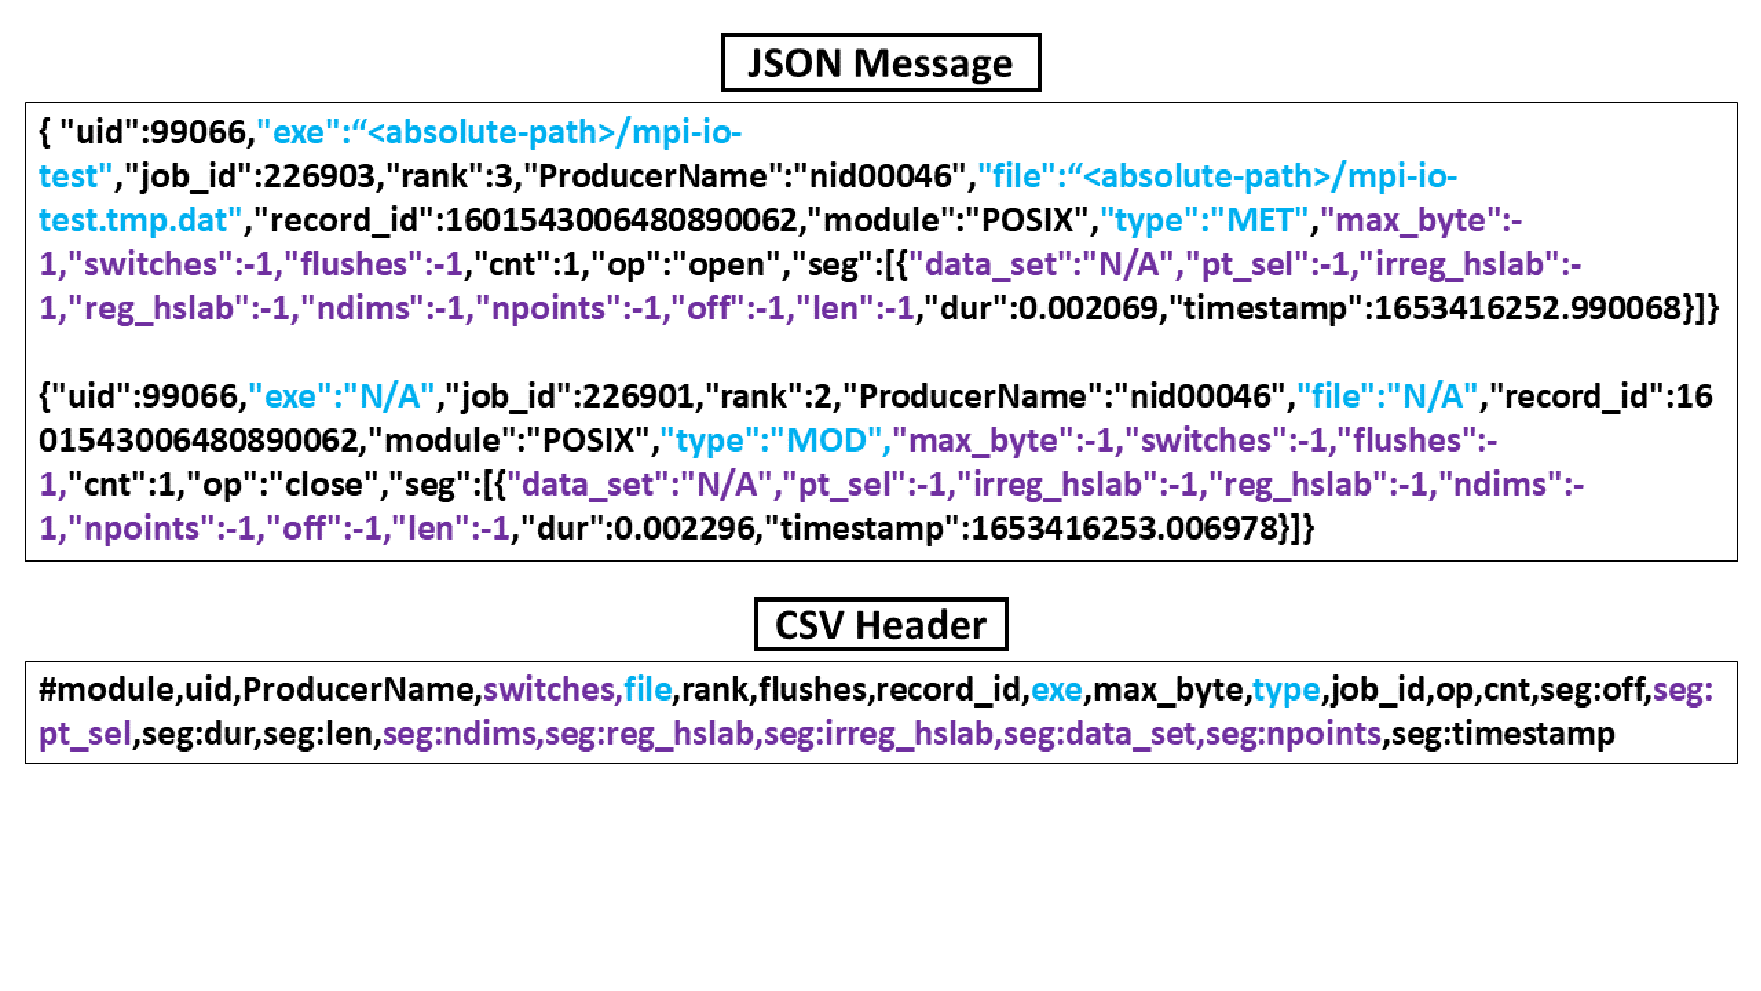
\includegraphics[trim={0 3cm 0 0},clip, width=1.01\linewidth]{figs/darshan-csv-json.pdf}
	\caption{Output of a MPI-IO Darshan test run in the JSON
          format (top image), and the CSV file header (bottom). 
          %The JSON message is published to the \emph{LDMS Streams}
          %interface where it is then converted to CSV and stored to
          %\emph{DSOS}. 
          The \texttt{name:value} pairs in light blue
          indicate meta data stored, while the light purple indicates
          the file level access data not applicable to POSIX. 
          %and are given the values of \texttt{"N/A"} or \texttt{"-1"}. 
          The \texttt{"seg"} is a list containing multiple \texttt{name:value} pairs.}
	\label{f:CSV Header and Output}
\end{figure}
Table \ref{table:metrics} depicts the names and definition of each
metric in the JSON file. Depending on the \texttt{"type"} input, the
absolute directory of the Darshan file output and executable will be
recorded and published to \emph{LDMS Streams}. If \texttt{"type"} is
set to \texttt{"MET"} (e.g. "meta"), the absolute directories will be
recorded. Otherwise, it will receive the value "N/A" if set to
\texttt{"MOD"}(e.g. "module"). The \texttt{"type"} will be set to
"MET" for open I/O events, which are the Darshan I/O records that have
permanent values during the application execution, such as the rank,
file and node name. The \texttt{"type"} is set to "MOD" for all other
I/O events to reduce the message size and latency when sending the
data through an HPC production system pipeline.

\begin{table*}[h]
  \centering
  \resizebox{\textwidth}{!}{
	\begin{tabular}{|l|l|}
	\hline
        \texttt{uuid} & User ID of the job run\\ \hline
	\texttt{exe} & Absolute directory of the application executable\\ \hline
	\texttt{module} & Name of the Darshan module data being collected\\ \hline
        \texttt{ProducerName} & Name of the compute node the application is running on\\ \hline
	\texttt{switches} & Number of times access alternated between read and write\\ \hline
	\texttt{file} & Absolute directory of the filename where the operations are performed\\ \hline
        \texttt{rank} & Rank of the processes at I/O\\ \hline
	\texttt{flushes} & Number of "flush" operations. It is the HDF5 file
                           flush operations for H5F, and the dataset flush
                           operations for H5\\ \hline
	\texttt{record\_id} & Darshan file record ID of the file the dataset belongs to\\ \hline
        \texttt{max\_byte} & Highest offset byte read and written per operation\\ \hline
	\texttt{type} & The type of JSON data being published: \texttt{MOD} for gathering module data or \texttt{MET} for gathering static meta data\\ \hline
	\texttt{job\_id} & The Job ID of the application run\\ \hline
	\texttt{op} & Type of operation being performed (i.e. read, write, open, close)\\ \hline
	\texttt{cnt} & The count of the operations performed per module per rank. Resets to 0 after each "close" operation\\ \hline
        \texttt{seg} & A list containing metrics names per operation per rank\\ \hline
	\texttt{seg:pt\_sel} & HDF5 number of different access selections\\ \hline
	\texttt{seg:dur} & Duration of each operation performed for
                           the given rank (i.e. a rank takes "X" time to perform a r/w/o/c operation)\\ \hline
        \texttt{seg:len} & Number of bytes read/written per operation per rank\\ \hline
	\texttt{seg:ndims} & HDF5 number of dimensions in dataset's dataspace\\ \hline
	\texttt{seg:reg\_hslab} & HDF5 number of regular hyperslabs\\ \hline
        \texttt{seg:irreg\_hslab} & HDF5 number of irregular hyperslabs\\ \hline
	\texttt{seg:data\_set} & HDF5 dataset name\\ \hline
	\texttt{seg:npoints} & HDF5 number of points in dataset's dataspace\\ \hline
        \texttt{seg:timestamp} & End time of given operation per rank (in epoch time)\\ \hline          
	\end{tabular}}
	\caption{Metrics defined in the JSON file published to the \emph{Darshan LDMS Integration}.}
	\label{table:metrics}
      \end{table*}

%\section{Additional Components}
%This section will provide a high level overview on how and why the \Darshan approach implemented the DSOS and Grafana tools for storage, analysis and visualization. 
\subsection{Storage: DSOS Database}
DSOS is built on the Scalable Object Store (SOS) database~\cite{sosgithub} and was intended to address the domain-specific needs of large-scale HPC monitoring. It was chosen as the preferred database because it allows for interaction via a command line interface which allows for fast query testing and data examination. DSOS also provides scalable data ingest and the ability to query large volumes of data which is required for the large amounts of data to be ingested and stored. %However, a different storage that had similar capabilities could be used instead. 
To sort though the published \emph{LDMS Streams} data, combinations of the job ID, rank and timestamp are used to create joint indices where each index provided a different query performance. An example of this is using \texttt{job\_rank\_time} which will order the data by job, rank then timestamp and then search the data by a specific rank within a specific job over time.

\subsection{Analysis and Visualization: HPC Web Services}
The HPC Web Services~\cite{ClusterAV} is an infrastructure that consists of the analysis and visualization components of this approach. Any data queries start from a front-end application and transferred to a back-end application that are running on an HPC cluster. In this case the front-end website is Grafana~\cite{grafana-website} and the back-end consists of Python analysis modules. The HPC Web Services also provide instant analysis where data can be analyzed and viewed in real time as opposed to the traditional method of querying the results of analyzed data from a separate database.

\begin{figure}
	\centering
	%\includegraphics[trim=0.2cm 8.5cm 12cm 0cm ,clip,width=0.9\linewidth]{figs/fig_kokkos_ldms.pdf}
	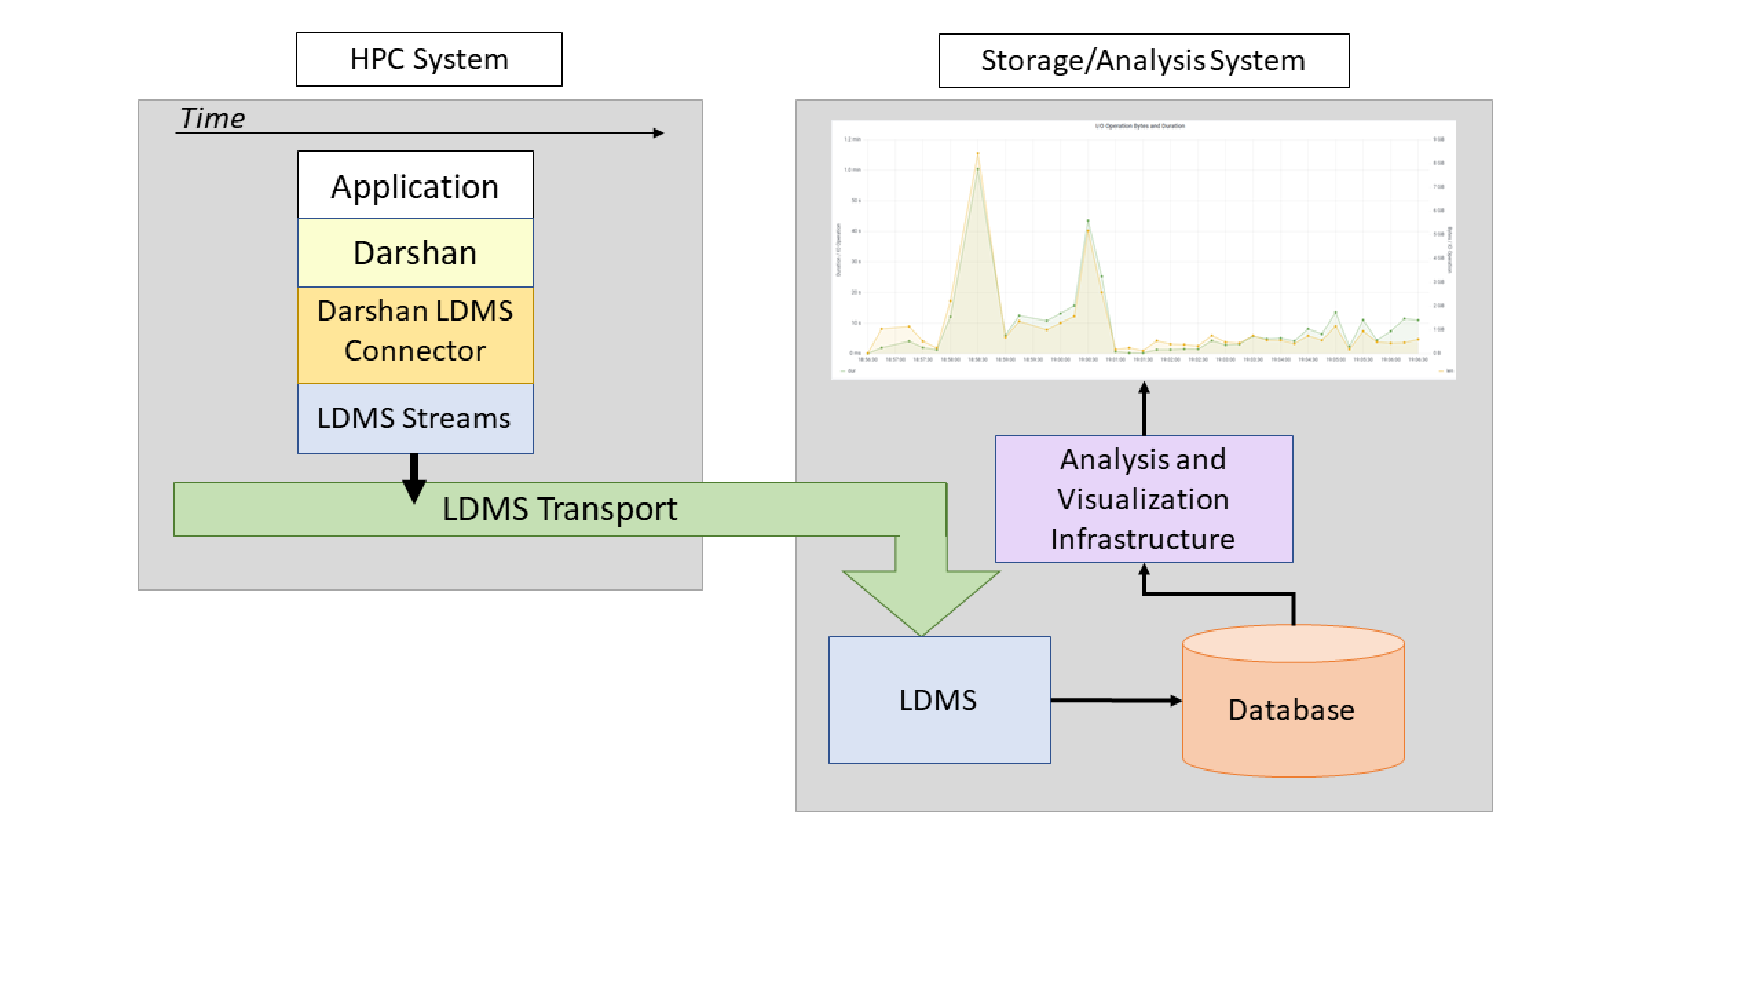
\includegraphics[trim=3cm 2cm 0cm 0cm, clip,width=1.2\linewidth]{figs/darshan-integration.pdf}
	\caption{Overview of the \Darshan where the \connector is used to intercept the I/O behavior Darshan is collecting utilizes the various tools to publish, store, analyze and view runtime I/O behavior.}
	\label{f:FrameworkOverview}
\end{figure}

Grafana is an open-source visualization application that provides various charts, graphs and alerts for supported data sources. It can support multiple data formats but is best suited for timeseries data. It has storage plugins for many database technologies in order to query and render data from multiple data sources. The \Darshan implemented a storage plugin for the DSOS database in order to query this data and visualize it on the Grafana web interface~\cite{grafana-website}. An overview of the this integration can be seen in Figure~\ref{f:FrameworkOverview}.

Python analysis modules are used to produce meaningful visualizations on the queried data from the DSOS database. With these modules, queried data is converted into a pandas dataframe to allow for easier application of complex calculations, transformations and aggregations on the data. The type of analysis module is specified in the Grafana web interface. This is where the \Darshan will demonstrate how runtime I/O data will provide further insights and understanding into application I/O behavior, patterns, performance variability and any correlations these have with the system behavior.   

%\RED{
	%\begin{itemize}
	%\item Explain how LDMS is integrated into Darshan. Give an overview on how we implement LDMS Streams into the Darshan DXT section to collect run time I/O data and push to a JSON file that then gets aggregated by LDMS and stored to SOS. Then explain how this stored data is then queried and displayed in a Grafana dashboard.
	%\item Add a pic of current Darshan LDMS integration setup (.png) 
	%\end{itemize}
	%}
